\documentclass{beamer}
%\usetheme{Madrid}
\usepackage[utf8]{inputenc}
\usepackage{dirtytalk}

\usepackage{pgf}
\usepackage{tikz}
\usetikzlibrary{arrows,automata}

\titlegraphic{\includegraphics[width=0.2\textwidth]{University_of_Pittsburgh_seal.png}}
\title{Project Proposal: Creating a Database of Definitions From Large Mathematical Corpora}
\subtitle{A comprehensive dictionary of all mathematical lexicon}
\author{Luis Berlioz\\
\texttt{lab232@pitt.edu}}
\institute{University of Pittsburgh}

\begin{document}
\begin{frame}
\titlepage
\end{frame}
\section{Objectives}
\begin{frame}{Project Objectives}
    \framesubtitle{What are we doing and why do we care about definitions}
\begin{itemize}
\item Find a comprehensive list of all the definitions used in Mathematics.
\item Organize them by meaning, dependency, etc.
\item Make it publicly available in the most useful format for machine learning practitioners.
\item \say{\textit{When one starts to delve into the language of mathematics, one encounters
        a phenomenon that is much more remarkable than the use of symbols. Mathematical language \emph{expands} as more mathematics is encountered.}} Mohan Ganisalengam
\end{itemize}
\end{frame}

\section{Data Pipeline}
%%%%FRAME
\begin{frame}{arXiv Website bulk download}
    \framesubtitle{All the \LaTeX{} source can be downloaded from an Amazon S3 bucket}
    \begin{columns}[T]
        \begin{column}{0.4\textwidth}
    \includegraphics[width=\textwidth]{bulk_download.png} 
        \end{column}
        \begin{column}{0.6\textwidth}
            \begin{itemize}
                \item About 885 Gigabytes of .tar files.
                \item Each .tar file is about 500 Megabytes.
                \item \texttt{arXiv\_src\_1806\_033.tar}
                    \begin{itemize}
\item \hspace{4em}      $\vdots$
\item 1806/1806.11561.gz
\item 1806/1806.11543.gz
\item 1806/1806.11557.pdf
\item 1806/1806.11567.gz
\item 1806/1806.11568.gz
\item \hspace{4em}      $\vdots$
\end{itemize}


            \end{itemize}
        \end{column}
    \end{columns}
\end{frame}

%%%%FRAME
\begin{frame}{LaTeXML}
    \framesubtitle{Process each article to get a more structured format}
    \includegraphics[width=0.9\textwidth]{ltxml_website.png}
    \includegraphics[width=0.9\textwidth]{ltxml_github1.png}
    \includegraphics[width=0.9\textwidth]{ltxml_github2.png}
\end{frame}

%%%%FRAME
\begin{frame}{Obtaining and Classifying Definitions}
    \begin{itemize}
            \item Sometimes the author of an article uses a \LaTeX macro to label a definition. These are our positive labels:
    \includegraphics[width=0.9\textwidth]{ltxml_defin_xml.png}
    \item To get negative labels, we pick paragraphs at random and assume they are not definitions.
        \item This has the drawback that some of the non--definitions are wrong.
    \item There are 1,707 articles in 2015 math.AG, we go from 5,229 labeled definitions to 71,067 ``probable'' definitions.  \end{itemize}
\end{frame}


%%%%FRAME
\begin{frame}{Some common metrics for Classification}
    \begin{itemize}
    \item Results using SVC in \textbf{scikit-learn}
    \includegraphics[width=0.7\textwidth]{class_results_svc.png}
    \item Sanity check:
    \includegraphics[width=0.95\textwidth]{sanity_check.png}
    \end{itemize}
    \begin{columns}[T]
        \begin{column}{0.5\textwidth}
     \includegraphics[width=0.8\textwidth]{def_appear_hist.png}
        \end{column}
        \begin{column}{0.5\textwidth}
    \includegraphics[width=\textwidth]{scatter_plot.png}
        \end{column}
    \end{columns}
\end{frame}

%%%%FRAME
\begin{frame}{Extracting the Definienda}
    \framesubtitle{Obtaining the data for Named Entity Recognition system}
    \begin{columns}[T]
        \begin{column}{0.5\textwidth}
    \includegraphics[width=\textwidth]{wiki_thin_banach.png}
        \end{column}
        \begin{column}{0.5\textwidth}
            \begin{itemize}
            \item Go through every of wikipedia article looking for a Definition section that contains the title.
            \item We obtain a pair: (\textbf{Definienda},  Definition).
            \item Just 5,321 matches out of almost 6 million articles.
            \item Several other website could be scrapped e.g. The Stacks project
            \end{itemize}
        \end{column}
    \end{columns}
\end{frame}

%%%%FRAME
\begin{frame}{Evaluating the NER Tagger} 
    \framesubtitle{Results of the BIO parser}
    \begin{columns}[T]
        \begin{column}{0.5\textwidth}
            \begin{tabular}{|c|c|r|}
                \hline
                \hline
        \multicolumn{2}{|c|}{\color{blue}{Input}} & \color{purple}{Output} \\
                \hline
                \hline
                \color{blue}{Token} & \color{blue}{POS} & \color{purple}{NER}\\
                \hline
                  We&PRP&O\\
                  \hline
                  define&VBP&O\\
                  \hline
                  a&DT&O\\
                  \hline
                  Banach&NNP&B--DFNDUM\\
                  \hline
                  space&NN&I--DFNDUM\\
                  \hline
                  as&IN&O\\
                  \hline
                  a&DT&O\\
                  \hline
                  complete&JJ&O\\
                  \hline
                  vector&NN&O\\
                  \hline
                  space&NN&O\\
                  \hline
            \end{tabular}
    \includegraphics[width=0.6\textwidth]{BIO_stats.png}
        \end{column}
        \begin{column}{0.5\textwidth}
            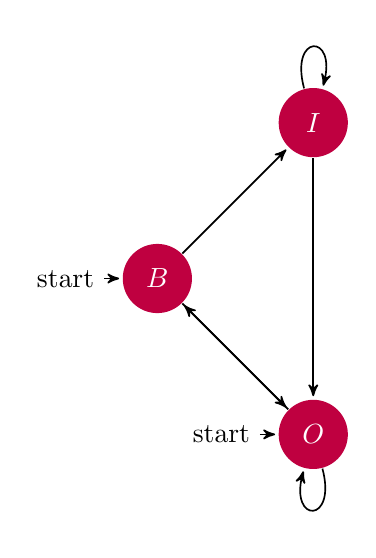
\begin{tikzpicture}[scale=0.5, ->,>=stealth',shorten >=1pt,auto,node distance=2.8cm, semithick ]
  \tikzstyle{every state}=[fill=purple,draw=none,text=white]

  \node[initial,state] (A)                    {$B$};
  \node[state]         (B) [above right of=A] {$I$};
  %\node[state]         (D) [below right of=A] {$q_d$};
  \node[initial,state]         (C) [below right of=A] {$O$};
  %\node[state]         (E) [below of=D]       {$q_e$};

  \path (A) edge              node {} (B)
            edge              node {} (C)
        (B) edge [loop above] node {} (B)
            edge              node {} (C)
        (C) edge [loop below]  node {} (C)
            edge               node {} (A);
\end{tikzpicture}

        \end{column}
    \end{columns}
\end{frame}

%%%%FRAME
\begin{frame} 
    \frametitle{Conclusions and Some Results}
    Some definitions found in the 2015 math.DG articles
    {\tiny\begin{tabular}{|l|l|}
        \hline
        almost flat manifold  &   An almost flat manifold whose 2-sylow subgroup of the holonomy group...\\
        \hline
        An infranilmanifold  &   An infranilmanifold is a double coset space \_inline\_math\_ where \_inli...\\
        \hline
        normal subgroup  &   Let \_inline\_math\_. Then \_inline\_math\_ is a normal subgroup of \_inline...\\
        \hline
        central involution  &   A central involution \_inline\_math\_ of an infranilmanifold \_inline\_mat...\\
        \hline
        infranilmanifold  &   Any infranilmanifold \_inline\_math\_ with \_inline\_math\_ a 2-group has a...\\
        \hline
        vector bundle  &   A vector bundle \_inline\_math\_ is flat if it has finite structure grou...\\
        \hline
        Tangent bundles of  &   Tangent bundles of infranilmanifolds are flat:...\\
        \hline
        infranilmanifold  &   Consider an infranilmanifold \_inline\_math\_. Note that \_inline\_math\_ i...\\
        \hline
        warped product  &   The warped product provides a way to construct new pseudo-riemannian...\\
        \hline
        Dualistic structures  &   Dualistic structures are closely related to statistical mathematics....\\
        \hline
        affine connection  &   In the notions of terms on statistical manifolds, for a torsion-free...\\
        \hline
        horizontal lift  &   Let \_inline\_math\_ in \_inline\_math\_. The horizontal lift of \_inline\_ma...\\
        \hline
    \end{tabular}}
    \begin{itemize}
            \item We believe that we have collected enough to believe that a robust collector of definitions from mathematical publications is possible.
            \item A lot of interesting work ahead:
                \begin{itemize}
                    \item Up until now we have ignored all math formulas and symbols.
                    \item Produce word embedding with math tokens (e.g. where smooth manifold is just one token).
                        \item Visualize the new terminology to assist with classification and dissambiguation.
                \end{itemize}
    \end{itemize}
\end{frame}
%%FRAME
\begin{frame}
\titlepage
\end{frame}
\end{document}

